\documentclass[]{final_report}
\usepackage{graphicx}
\usepackage{hyperref}
\usepackage{listings}


%%%%%%%%%%%%%%%%%%%%%%
%%% Input project details
\def\studentname{Ciaran Palmer}
\def\projecttitle{SensorML on SenseTile}
\def\supervisorname{Your Supervisor Name}
\def\moderatorname{Your Moderator Name}


\begin{document}

\maketitle
\tableofcontents\pdfbookmark[0]{Table of Contents}{toc}\newpage

%%%%%%%%%%%%%%%%%%%%%%
%%% Your Abstract here

\begin{abstract}
SenseTileSensor Board

SensorML description.

WebServer to access sensor observations

SensorML Bon Mapping with a tool and method to develop sensorML descriptions

\end{abstract}




\newpage


%%%%%%%%%%%%%%%%%%%%%%
%%% Acknowledgments

\chapter*{Acknowledgments}


%%%%%%%%%%%%%%%%%%%%%%
%%% Introduction

\chapter{Introduction}

The aim of this thesis project was to model the SenseTile Sensor Board using Sensor Model Language (SensorML)\cite{SensoMLref} . A prototype of a Web Service for accessing SenseTile Sensor Board sensor observations was to be developed using this SensorML description of the SenseTile Sensor Board. An evaluation of the suitability of SensorML for use as part of the SenseTile System was also to be performed.

SenseTile is a sensor and processing package including motion sensors, RFID sensors, temperature sensor, audio sensors, pressure sensors, light level sensors video sensors among others. It is used as a replacement for standard ceiling tiles to provide smart building services as part of a Web Sensor Network. The SenseTile System is made up of two units a Sensor Board and Processor Unit. The sensors are interfaced or hosted on the Sensor Board. The Processor Unit interfaces to the Sensor Board allowing data from the Sensor Board to be processed futher as required.

SensorML is one of a number of specifications provided by the Open Geospatial Consortium (OGC) as part of the Sensor Web Enablement(SWE) initiative[ref]. The members of the OGC have the goal of developing open standards to exploit Web connected sensors of all types. SensorML is used to describe sensor systems and the processing of sensor observations. It provides standard models and XML encodings to describe the process of sensor measurement. SensorML is described further in chapter x.

The SenseTile Web Service prototype allows access to the Sensor Board sensor observations and it's SensorML description. It runs on the SenseTile Processor Unit.  The Web Service is based on another OGC SWE  specification, the Sensor Observation Service (SOS)[ref]. This specification defines a standard Web interface for retrieving information about sensor systems and sensor observations. Sensor Board measurements that have been post processed and converted to real values or the raw Sensor Board data can be accessed using the Web Service. SOS Lite.

There are othe  SOS specification depend on another SWE specification, Observation and Measurements(O\&M)[ref]. This specification provides standard models and XML encoding for sensor observations.

A  SensorML to BON Mapping was also to be explored . BON\cite{BONref} is a notation and a method for Object Oriented systems analysis and design. Based on this mapping it was proposed to develop a tool/method to automatically generate SensorML descriptions. Generally SensorML is hand generated with all the shortcomings of such an approach. The proposed approach would allow sensor processing to defined formally in BON and then refined to JML/Java. 


\chapter{ Background Research}


\section{Sensor Web Enablement}
The Open Geospatial Consortium (OGC) Sensor Web Enablement (SWE) [ref]  is establishing interfaces and protocols that will enable a standardised Sensor Web. It is hoped that an easier integration and development of sensor applications across sensor networks will be facilitated by this standarising activity.The OGC SWE provides a framework of open standards for use with Web-connected sensors and sensor systems. There are seven main specifications currently:

\begin{itemize}
\item  SensorModel Language(SensorML) - models and schema for sensor systems and processes surrounding measurements
\item  Observations \& Measurements (O\&M) - models and schema for packaging observation values
\item  Transducer Markup Language (TML) - models and schema for multiplexed data from sensor systems
\item  Sensor Observation Service (SOS) - standard web interface for accessing observations
\item  Sensor Planning Service (SPS) - standard web interface for tasking sensor systems and model and requesting acquisitions
\item   Sensor Alert Service (SAS) - standard web interface for publishing and subscribing to sensor alerts
\item   Web Notification Service (WNS) - standard web interface for asynchronous notification
\end{itemize}
There is also the SWE Common that provides common data models and schemas for the above.

Rather than define any new sensor models or XML formats for SenseTile it preferable to use the existing solutions if good enough for the task at hand. The SWE framework seems to cover all needs for modeling sensors and observations. Support the use of Web Services is the main rational and fits the needs of a SenseTile Sensor Network. In this case the SOS and SensorML are core.

Scalable - can be  large systems. Discovery. Process data without having to define an implementation as this
can be provided as part of SensorML description.

 DAML?

\section{Sensor Modeling Language}
Sensor Modelling Language (SensorML) is used to describe sensor systems and the processing of observations from sensor systems.

The purposes of SensorML are:
\begin{itemize}
\item Provide sensor and process information in support of resource and observation discovery
\item Support the processing and analysis of the sensor observations
\item Support the geolocation of observed values (measured data)
\item Provide performance characteristics (e.g., accuracy, threshold, etc.)
\item Provide an explicit description of the process by which an observation was obtained (i.e., it’s lineage)
\item Provide an executable process chain for deriving new data products on demand (i.e., derivable observation)
\item Archive fundamental properties and assumptions regarding sensor systems
\end{itemize}

SensorML provides a functional model of sensors and an XML encoding to describe sensors and their observations.
Sensors are modelled as processes that convert real phenomena to data. Processes take inputs, process them and result in one or several outputs.

Sensor metadata is also supported by SensorML.  

The processes can be connected together in chains using SensorML ProcessChains or Systems. 

including measurement by a sensor system, as well as post-measurement
processing.

When Modeling a sensor system in SensorML the main entities used are Systems and Components. 

A SensorML System is used to group sensors that are related spatially to one another.  As it is a process chain it is hierarchical and so Systems can contain Systems.

A Component is an atomic process that generally converts a physical phenomena to a digital number. 

ProcessModels are another modeling that is used to describe a pure process that has no physicality. They point to an implementation or a description of one.

The data types used for inputs and out puts come another OGC sepc the SWE common. Examles are Quantity which is a decimal number, Count, Boolean, Category, and Time provide the basic primitives. Within SensorML, 

Aggregation of primitive data types are also provided DataRecord or DataArray.

A sensor systems would likely to be based mainly on Systems and
Detector model. Reference tutorial and sensorml specification.

The SensorML description of the SenseTile Sensor Board is described in chapter .

\section{Sensor Observation Service}
The SenseTile Web Service is based on the concepts described in the Sensor Observation Service (SOS) specification. The SOS defines a web service interface for the discovery of sensors systems and the retrieval of observations from sensor systems.  Observations are encoded as OGC O\&M Observations. Sensor systems metadata can be also be retrieved using the SOS interface and is generally defined in SensorML or TML.
para. An SOS organizes collections of related sensor system observations into Observation
Offerings. These operations are encoded in XML and used in http post and get operations. The XML message needs to be parsed to identify the operations, parameters and results. There seems to be work ongoing to change this to a more industry standard view of Web Services with the use of WSDL/SOAP. I could not find this as part of current OGC SWE framework.
para: Scalability would be achieved through aggregating a number of
sensor data producers on the sensor side and by aggregating a number of SOS instances
on the data center side for providing data to consumers. 
\subsection{SOS Data Consumer Operations}
There are there core operations that are provided by an SOS and used by SOS Clients to request sensor information:
 \begin{itemize}
\item GetObservation operation is used to obtain sensor observations and measurement data.
\item GetCapabilities operation is used to retrieve SOS service metadata.
\item DescribeSensor operation retrieves detailed information about the sensors .
\end{itemize}

\subsection{SOS Data Provider Operations}
Two other operations RegisterSensor and InsertObservation are of interest to this thesis . These are part of the SOS transactional interface. They are used with SOS data producers which are software entities connected to the sensor and have enough processing power to generate XML descriptions of the sensor data.

\subsection{SOS Catalogs}
The catalog aspect of SOS that used for discovery of the SOS instance is not covered in the Web Service Prototype described in this thesis. 
\subsection{Enhanced Operations}
Also six enhanced operations, GetResult,
GetFeatureOfInterest, GetFeatureOfInterestTime, DescribeFeatureOfInterest,
DescribeObservationType, and DescribeResultModel are not included in the SenseTileWeb Service.

\section{OGC Lib}
The VAST Team at the University of Alabama in Huntsville (UAH)  developed an open source JAVA framework call swe-common-data-framework (http://code.google.com/p/swe-common-data-framework/) to allow the quick development of SWE services such as an SOS. In this project the library is used for it's SensorML parsing and SensorML process execution functionality.
\section{UCD Sensor Board library}
UCD Research group providing a Java lib to access the data 
\section{BON}
\section{JAXB}
\section{AXIS 2.0}


\chapter{Design}
\section{SensorML Description of SenseTile}

A SensorML model of SenseTile was developed as part of this thesis. The model contains metadata about the SenseTile system and supports the needs of the SenseTile Web Service. Two main requirements of the SenseTile Web Service were to be supported by the SensorML model. Firstly the raw data from the senors was to be retievable to allow external system process the data as desired. Secondly there was a requirement to do post processing on the Processor Unit of the sensor data to convert it to meaningful values.

A block diagram of the Sensetile SensorML model is shown in figure \ref{fig:SenseTileSystem}.
\begin{figure}[h]
\scalebox{0.70}{\includegraphics{SenseTileSystem.png}}
\caption{SenseTile System Block Diagram}\label{fig:SenseTileSystem}
\end{figure}

Three SensorML Systems are used to model the SenseTile system. One SensorML System models the overall SenseTile System and connects the other two SensorML Systems used, the Sensor Board System and the Conversion System. The physical phenomena measured by the sensors are the input to the  SenseTile System. These values will be read in from packets received from the Sensor Board. The Digital Number output is the raw sensor data which is a digital number without a physical meaning. The Converted Measurement output contains the values from post processing the sensor data which have some physical meaning such as temperature in Celcius.

The division of the systems is based on the concept that sensor observations are based on at least a sampling process and a conversion process{ref tutorial}. The Sensor Board System contains SensorML Components that model the sensors on the board that perform the sampling while the SensorML Components contained in the Conversion System model process that produce meaningful physical measurement values such as temperature and lumens.

A block diagram of the Sensetile SensorML model with Components is shown in figure \ref{fig:SensorML_SenseTile_System_comp}. Only the Thermistor Component and the Celcius Component are developed as part of this thesis. They are described in model detail in later sections.
\begin{figure}[h]
\scalebox{0.65}{\includegraphics{SensorML_SenseTile_System_comp.png}}
\caption{SenseTile System Components}\label{fig:SensorML_SenseTile_System_comp}
\end{figure}

Naming rules for inputs and outputs - allow more generic handling of implementation classes.

System and components are in several files. Inline in one file if desired.

\subsection{Thermistor Component}
The SensoML Thermistor component contains the metadata for the Sensor Board Thermistor x. It's temperature input is modeled using a quantity value without any units as is a measured phenomena. Its output is a digital number from the sensor.

contraints.

fragment
\subsection{Celcius Converter Component}

The SensoML Celcius Converter component performs a conversion of the Thermistors digital number output to a real quantity celcius value. 

make portable
formula

\newpage
\section{BON to SensorML mapping}
Features to be elements or attributes.

Name rule suffix "Attrib" to make it an attribute.

List handling - convention for mapping.

SML prefix to handled key word clashes between sensorML and BON.


\section{SenseTile Web Service}
\subsection{Overview}

The SenseTile Web Service is based on the Sensor Observation Service (SOS) as described previously. The two main entities in the SOS, the Sensor Data Provider and the SOS,  are used to structure the SenseTile Web Service. The two entities are implemented as seperate software component that together provide the service. The Sensor Data Provider component will be referred to as the DataProvider in this design.

The two components are run as seperate processes on the SenseTile processor unit to allow a more flexible network architecture.  This network architecture is described in more detail in section. The basic system structure is shown in figure \ref {fig:Deployment_sensetile} .

\begin{figure}[h]
\scalebox{0.65}{\includegraphics{Deployment_sensetile.png}}
\caption{SenseTile Web Service}\label{fig:Deployment_sensetile}
\end{figure}

The DataProvider will be configured with a SensorML description of the SenseTile System, read sensor data form the Sensor Board and provide these as O\&M Observations to the SOS. The SenseTile SOS will implement the SOS core operations to allow a client to get the observations. The following sections describe the design of the DataProvider and SOS components as well as the scenarios they support.

\subsection{Supported Scenarios}
\begin{table}[!th]
\begin{tabular}{|l|c|r|}
\hline
Scenarios\\
\hline
Generate Observations from Sensor Data \\
\hline
Get Sensor Description from SOS\\
\hline
Get  Sensor Observation from SOS\\
\hline
\end{tabular}
\caption{Scenario Chart for SenseTile Web Service}
\label{ex:table}
\end{table}
\subsection{SenseTile WebService Network Architecture}
In this prototype there is a divergance from how the SOS is envisoned to be implemented. In the SenseTile Web Service the SOS runs on the Processor Unit to allow access to the sensor data directly from the SenseTile rather than on a external large server. 
\begin{figure}[h]
\scalebox{0.65}{\includegraphics{Deployment_sensetile_network.png}}
\caption{SenseTile Web Service}\label{fig:Deployment_network}
\end{figure}
\begin{figure}[h]
\scalebox{0.65}{\includegraphics{Deployment_sensetile_ext_sos.png}}
\caption{SenseTile Web Service}\label{fig:Deployment_ext_sos}
\end{figure}
\begin{figure}[h]
\scalebox{0.65}{\includegraphics{Deployment_sensetile_sos_aggr.png}}
\caption{SenseTile Web Service}\label{fig:Deployment_sos_aggr}
\end{figure}
It is envisioned that the SOS does not need to be run on every Processor Unit. Several SenseTile could excute just the DataProducer software and be configured with the address of the SOS to use.



\subsection{DataProducer}

DataProducer generates observations in Observation xml standard.

Interface to the SensorBoard Library.

Uses observer pattern to update sensors with packets from the board.

reads sensors from SensorBoard System xml

Sensors iimplement interface to facilitate this.

Vast lib connects all the processes

implementation of sensor and convertor is named using URN read from the sensorMl descption.


The DataProducer was developed as a SensorML based software. It would be parse the SenseTile SensorML model to instantiate the code to excute the processes described. This required two aspects to be developed, a framework to run the processes and classes that implemented the components.

\begin{figure}[H]
\scalebox{0.65}{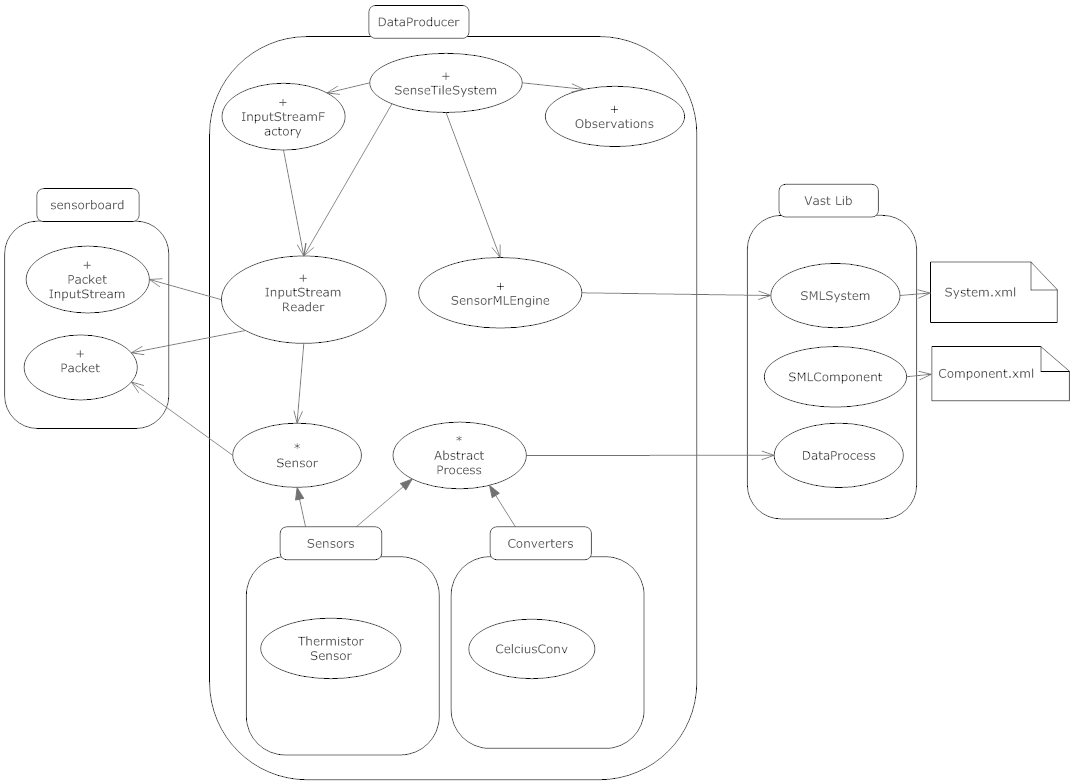
\includegraphics{sensetile_static_diagam.png}}
\caption{DataProducer Static Diagram}\label{fig:sensetile_static_diagam.png}
\end{figure}

Interfaces to the Sensor Board
Use PacketInput stream to access SenseTile observation packets.

\subsubsection{Sensors}

Thermistor components reads out the temperature value
and its output is sent to both the raw data and the celcius
converter component and on to the tuples. System reads packets
and averages them for every configurable seconds. Default 1.
These tuples are sent to webservice provider as observations.

Observation as described in SOS.


\subsection {SOS}
 \begin{figure}[h!]
\scalebox{0.65}{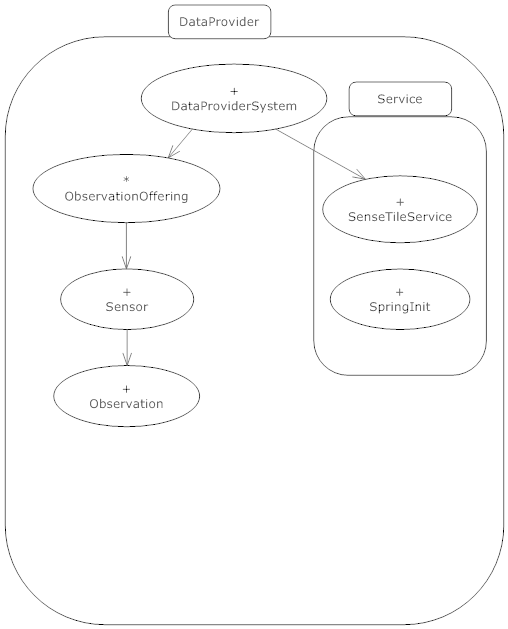
\includegraphics{bon_static_diagam_provider.png}}
\caption{SOS Static Diagram}\label{fig:bon_static_diagam_provider.png}
\end{figure}
Keeps track of sensorboards that register

provides an RMI interface to the DataProducer to update with observations. This has lower overhead
than a web service. Though it would not be hard to change to use a Web Service Interface.

GetObservaton - marshal Observation to xml string and send as response.

StreamObservation -  registered clients get new observation sent over UDP connection?

Provides a Web Service interface  based on Sensor Observation Service. Not fully as is a very complex interface.

\newpage
\section{SensorML generation}

Java binding wth JIBX  generate sensorml.

Simple xml file with Sensor metadata.

Naming rules allow connection of inputs and outputs
in sensorML processes.

 component id +Input

 component id+Output

\chapter{ Detailed Design and Implementation}

\section{DataProducer}

DataProducer VastLib UCD SenseTile Driver Lib

\section{SOS}
 is based on AXIS 2.0/Spring

JAXB for SensorML XML to java binding.

RMI used between DataProvider and SOS.

\section{SensorML Generation}

\chapter{Results}

running prototype tested with UCD SensorBoard Simulator code

Tested against real SenseTile and sensor data retrieved by a testclient.

Generation of SensorML description of a Senstile Sensor

\chapter{ Conclusions and Future Work}

what has been achieved

the weaknesses of your approach
SOS on the Processor Board. Is this right.

difficult schemas to program against.
JIBX did not generate a default binding.
Jaxb did with some help but did not generate the process type correctly.
Why?

Schemas cover all needs for sensor description and data.

SWE not fully web services as W3C might define. Not SOAP. HTTP envelope
flexible.
Streaming the data.

\chapter{References}
\newpage
\begin{thebibliography}{99}
\bibitem{SensoMLref}Open Geospatial Consortium Inc., OpenGIS Sensor Model Language (SensorML) Implementation Specification, 2007
\bibitem{SOSref}Open Geospatial Consortium Inc., OpenGIS  Implementation Specification, 2007
\bibitem{OMref}Open Geospatial Consortium Inc., OpenGIS  Implementation Specification, 2007
\bibitem{SWEArchref}Open Geospatial Consortium Inc., , 2007
\bibitem{SMLTutorialref}Open Geospatial Consortium Inc., , 2007


\bibitem{BONref}Kim Waldén and Jean-Marc Nerson , "Seamless Object-Oriented Software Architecture", 1995
\end{thebibliography}
\label{endpage}


\chapter{Appendices}

\lstset{language=XML,basicstyle=\small}
\lstinputlisting{Thermistor.xml}





\end{document}

\end{article}
